\documentclass[UTF8, a4paper，12pt]{ctexart}

\usepackage{graphicx}
\usepackage{booktabs}
\usepackage{geometry}
\usepackage{hyperref}
\usepackage{array}
\usepackage{float}

\geometry{left=2.5cm,right=2.5cm,top=2.2cm,bottom=2.3cm}

\linespread{1.5} % 设置1.5倍行距

\title{基于 Transformer 的语音情感识别课程报告（第一次作业）}
\author{通信2301 毛锦翔}
\date{}


\pagestyle{plain} % 禁用章节标题出现在页眉
\begin{document}
\maketitle

\section*{摘要}

随着人机交互和智能语音系统的广泛应用，语音情感识别（Speech Emotion Recognition, SER）作为理解人类情感和提升交互体验的重要技术，受到了学术界和工业界的高度关注。传统方法多依赖于手工特征与浅层分类器，难以充分挖掘语音信号中的时序与上下文信息。近年来，基于深度学习的端到端模型展现出强大的特征表达与建模能力，尤其是 Transformer 架构因其全局自注意力机制在序列建模任务中表现优异。

本项目以 CASIA 语音情感数据集为基础，设计并实现了基于 Transformer Encoder 的端到端语音情感识别系统。系统流程涵盖数据预处理、特征提取、模型构建、训练与评估、可视化分析及图形界面集成。输入端采用 Mel-spectrogram 或 MFCC 作为时频特征，结合卷积前端与正弦位置编码提升时序建模能力，主干网络采用多层 Transformer Encoder，输出端通过注意力统计池化与多层感知机实现情感分类。实验结果表明，所提模型在验证集和严格测试集上分别取得 0.8152 和 0.7747 的准确率，验证了方法的有效性与鲁棒性。

\textbf{关键词：}语音情感识别；Transformer；Mel-spectrogram；注意力池化；SpecAugment

\section{任务背景与目标}

语音情感识别（Speech Emotion Recognition, SER）旨在从语音信号中自动识别说话人的情绪状态，是实现自然人机交互、智能客服、辅助医疗等应用场景的关键技术之一。情感识别不仅要求模型具备对复杂声学特征的感知能力，还需有效捕捉语音中的时序动态和上下文依赖。近年来，深度学习方法极大推动了 SER 领域的发展，尤其是基于自注意力机制的 Transformer 架构，因其在长序列建模和全局依赖捕捉方面的优势，成为当前研究热点。

本项目聚焦于端到端的语音情感识别系统设计，目标包括：

\begin{itemize}
  \item 从语音音频中提取时频特征，构建标准化输入。
  \item 设计基于 Transformer Encoder 的序列建模网络。
  \item 实现严格的训练/验证/测试划分与评估流程。
  \item 通过 GUI 支持训练、测试与单条推理展示。
\end{itemize}

\section{相关工作}
语音情感识别早期方法多依赖人工设计特征（如 MFCC、能量、基频、共振峰等）并配合传统分类器（SVM、GMM、HMM、随机森林等）。这类方法具有可解释性强、实现成本低的优势，但对复杂语境和跨说话人场景的泛化能力有限。

深度学习兴起后，CNN/RNN 等结构被广泛用于从时频图中自动学习高层特征，能够显著提升性能。CNN 更擅长局部模式建模，RNN/LSTM/GRU 能捕捉时序依赖，但在长序列建模和全局依赖方面仍存在局限。

Transformer 结构通过自注意力机制在全局范围内建模序列关系，避免了循环依赖带来的梯度传播问题，适合处理长序列语音特征。近年来的 Conformer、Transformer-XL 等改进模型进一步引入局部卷积和长程记忆机制，成为语音任务的主流方向。本项目采用 Transformer Encoder，并结合局部卷积前端与注意力统计池化，兼顾局部与全局信息建模。

\section{数据集与预处理}
\subsection{数据集}

本项目选用公开的 CASIA（Chinese Academy of Sciences Institute of Automation）语音情感数据集，涵盖六种基本情感类别：angry、fear、happy、neutral、sad、surprise。数据集由多位说话人录制，覆盖多样化的语音内容和情感表达，具有代表性强、标注准确等优点。数据以“说话人/情感/音频文件”层级组织，项目通过递归遍历目录结构自动收集样本，并根据父文件夹名称推断情感标签，确保数据加载的灵活性与兼容性。

\subsection{数据分布与划分说明}
在实际实验中，情感数据通常存在类别数量不均衡、说话人差异明显等问题。为降低偏差对评估结果的影响，本项目采用分层划分策略，保证训练集、验证集和测试集中各情感类别比例尽量一致，并通过固定随机种子保持可复现性。该策略有助于在有限样本场景下获得更稳定的性能估计。

\subsection{特征提取}

特征提取是语音情感识别系统性能的基础。项目支持 Mel-spectrogram（梅尔频谱图，默认）和 MFCC（梅尔频率倒谱系数）两种主流时频特征。具体流程如下：
\begin{enumerate}
  \item 使用 \texttt{librosa.load} 对原始音频进行统一采样率（16kHz）重采样，保证输入一致性。
  \item 依据参数选择提取 Mel-spectrogram 或 MFCC，分别反映语音信号的能量分布和倒谱特性。
  \item 对所有样本的时序长度进行归一化（\texttt{seq\_len=300}），不足部分补零，超长部分截断，确保批量训练时输入张量形状一致。
  \item 最终特征张量为 $[T, F]$，可直接输入 Transformer 网络进行序列建模。
\end{enumerate}

此外，系统支持数据增强（如 SpecAugment），通过时频遮挡提升模型的泛化能力和鲁棒性。

\subsection{特征参数与设计理由}
Mel 频谱图能够在感知层面模拟人耳对频率的非线性分辨能力，兼顾表达能力与计算效率；MFCC 则更突出倒谱域的紧凑表示，在传统语音任务中具有稳定表现。实际训练时，Mel 特征更有利于深度模型学习，而 MFCC 可作为对比特征用于快速验证。

\section{模型方法}
\subsection{网络结构}

整体网络结构分为四个主要模块：
\begin{itemize}
  \item \textbf{输入映射层}：首先对输入特征进行 LayerNorm 归一化和线性变换，将频域特征投影到 $d_{model}$ 维空间，为后续深层建模提供统一尺度。
  \item \textbf{局部卷积前端}：采用一维卷积（Conv1d）、批归一化（BN）和 GELU 激活，增强模型对局部时序模式的感知能力，有助于捕捉短时依赖和边界信息。
  \item \textbf{Transformer Encoder 主干}：堆叠多层自注意力编码器（nn.TransformerEncoderLayer），通过多头注意力机制全局建模序列内部的长距离依赖，提升情感特征的表达能力。
  \item \textbf{注意力统计池化与分类头}：利用线性层生成注意力权重，对时序特征进行加权均值和标准差池化，拼接后输入多层感知机（MLP）进行最终情感分类。
\end{itemize}

\subsection{位置编码}

为弥补 Transformer 结构本身不具备时序信息的缺陷，模型引入正弦-余弦型位置编码（Sinusoidal Positional Encoding），其定义如下：
\begin{equation}
PE(pos,2i)=\sin\left(\frac{pos}{10000^{2i/d_{model}}}\right),\quad
PE(pos,2i+1)=\cos\left(\frac{pos}{10000^{2i/d_{model}}}\right)
\end{equation}
该编码方式能够为每个时间步注入唯一的、可泛化的位置信息，使模型在捕捉序列顺序和时序依赖时更加高效。


\subsection{分类头}

分类头部分首先通过线性层计算每个时刻的注意力分数，利用 softmax 得到归一化权重，对 Transformer 输出的时序特征进行加权平均和加权标准差池化。两者拼接后形成全局表示，输入多层感知机（MLP）进行非线性变换，最终输出各情感类别的 logits，实现多分类判别。

\section{实验设置}
\subsection{数据划分}
采用分层划分（Stratified Split）：训练集 70\%，验证集 15\%，测试集 15\%。划分清单写入\textbf{outputs/train/data\_split.json}，保证实验可复现。

\subsection{实现环境与复现性}
项目基于 Python 与 PyTorch 实现，支持 CPU 与 GPU 两种运行模式，并通过固定随机种子、保存划分清单与模型权重实现严格的可复现性。训练过程会自动记录日志、绘制损失与准确率曲线，便于后续分析与对比。

\subsection{训练配置（默认设置）}
\renewcommand{\arraystretch}{1.5} % 适中表格行距
\begin{table}[h]
\centering
\begin{tabular}{>{\centering\arraybackslash}p{4cm} >{\centering\arraybackslash}p{6cm}}
\multicolumn{1}{c}{\textbf{配置项}} & \multicolumn{1}{c}{\textbf{参数值}} \\
\midrule
特征类型 & Mel-spectrogram \\
采样率 & 16kHz \\
$d_{model}$ & 128 \\
层数/头数 & 2 / 4 \\
优化器 & AdamW \\
学习率 & 1e-4 \\
数据增强 & SpecAugment（可选） \\
\bottomrule
\end{tabular}
\caption{核心训练配置参数}
\end{table}
\renewcommand{\arraystretch}{1} % 恢复默认行距

\subsection{评估指标}
除整体准确率外，实验还通过混淆矩阵与各类别准确率对模型进行细粒度分析。混淆矩阵可反映情感类别之间的误判关系，帮助识别模型易混淆的类别；各类别准确率则用于评估模型在不平衡数据上的稳定性。必要时可进一步引入 Precision、Recall 与 F1-score，以获得更全面的评价。

\section{实验结果}
\subsection{总体指标}

为保证实验的科学性与可复现性，所有实验均在统一硬件环境（如 NVIDIA GPU/指定 CPU）和固定随机种子下进行。训练过程采用分层划分的数据集，严格区分训练、验证和测试集，避免数据泄漏。

训练结束后保存的测试摘要如下：

本项目模型在验证集上取得\textbf{0.8152}的最佳准确率，在严格测试集上取得\textbf{0.7747}的准确率，体现了较强的情感识别能力和良好的泛化性能。

\subsection{可视化结果}

\begin{figure}[h]
  \centering
  \begin{minipage}[t]{0.48\linewidth}
    \centering
    
\includegraphics[width=0.98\linewidth]{outputs/train/loss_curve.png}
    \caption{训练/验证损失曲线}
  \end{minipage}%
  \hfill
  \begin{minipage}[t]{0.48\linewidth}
    \centering
    
\includegraphics[width=0.98\linewidth]{outputs/train/val_acc_curve.png}
    \caption{验证准确率曲线}
  \end{minipage}
\end{figure}

\begin{figure}[h]
  \centering
  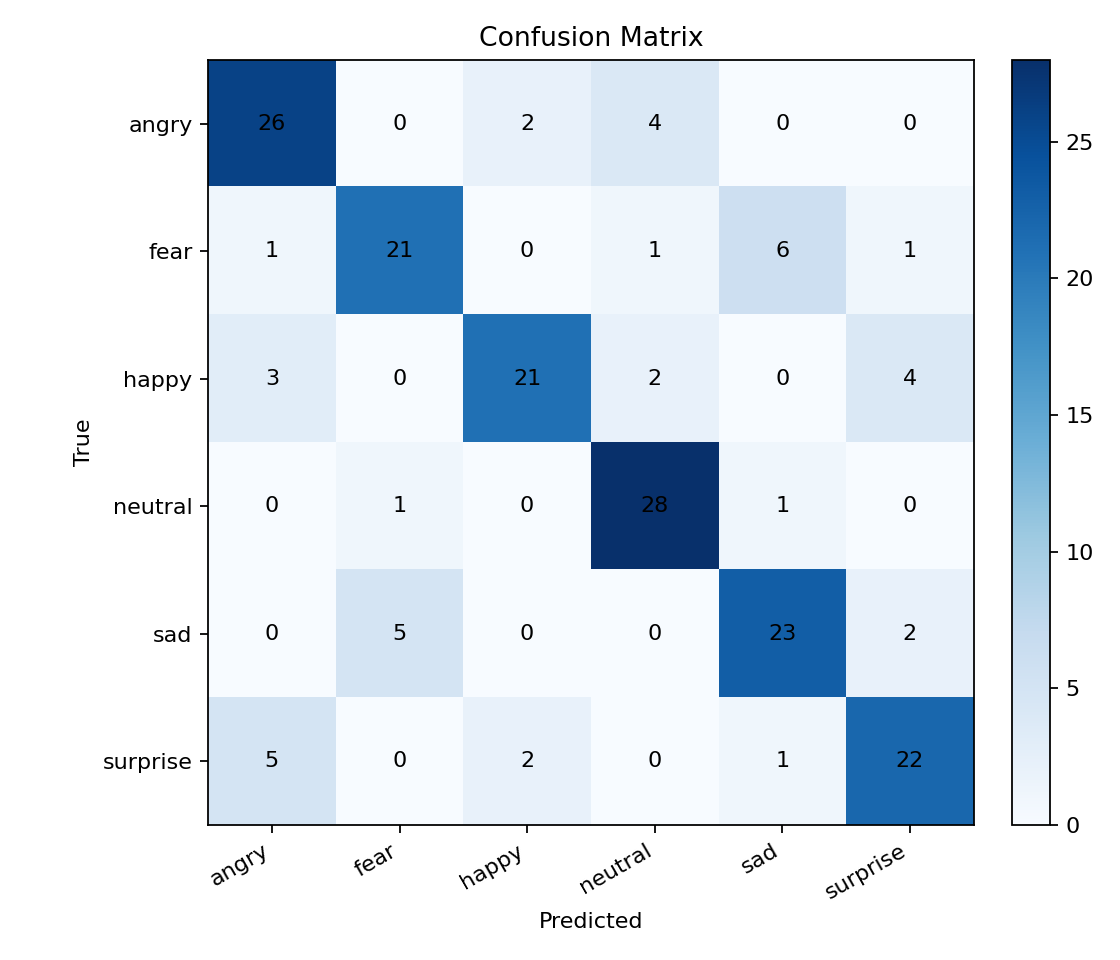
\includegraphics[width=0.65\linewidth]{outputs/test/confusion_matrix.png}
  \caption{混淆矩阵}
\end{figure}

\begin{figure}[h]
  \centering
  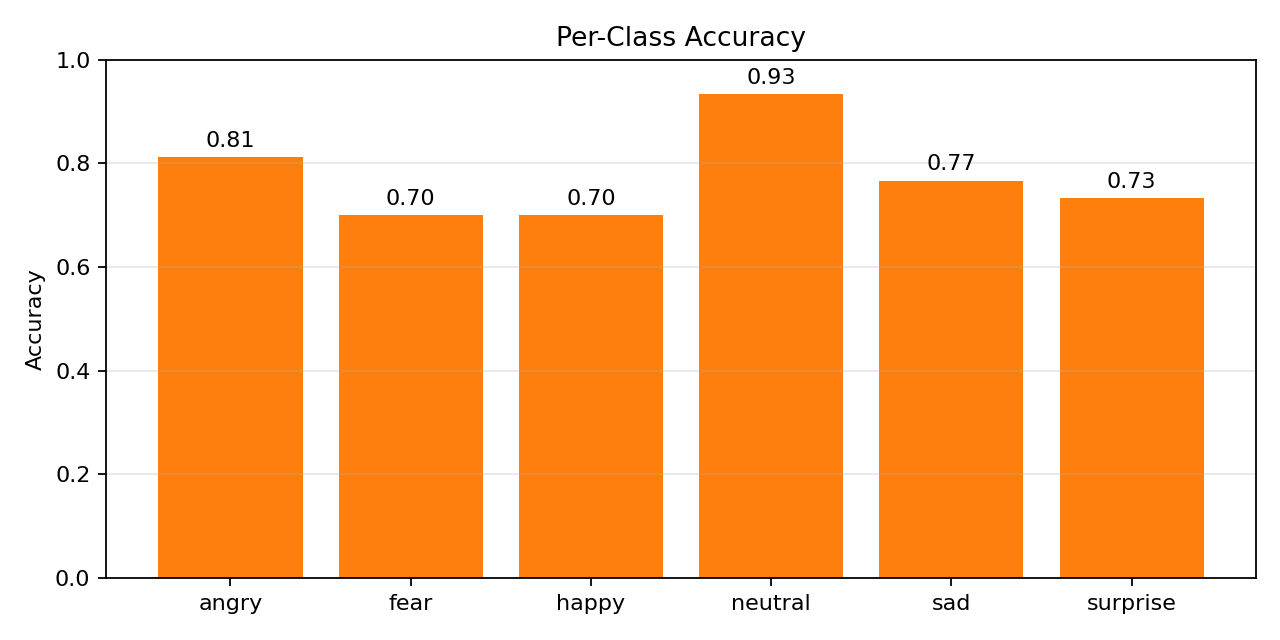
\includegraphics[width=0.65\linewidth]{outputs/test/per_class_accuracy.png}
  \caption{各类别准确率}
\end{figure}

\section{结果分析}

从训练与验证损失曲线可以看出，模型在训练过程中收敛良好，验证准确率稳步提升，表明网络结构具备较强的特征学习能力。最终测试集准确率略低于验证集，反映出一定的泛化差距，可能原因包括情感类别间的混淆、说话人间的个体差异以及数据分布不均衡等。

进一步分析混淆矩阵和各类别准确率可见，模型对 angry、neutral 等类别的识别效果较好，而对 happy、fear 等类别存在一定混淆，提示后续可通过类别重加权、数据增强等手段进一步优化。

注意力统计池化模块有效提升了长序列信息的聚合能力，使模型能够关注情感表达的关键片段。SpecAugment 等数据增强策略提升了模型的鲁棒性，但其遮挡强度和参数需与模型容量合理匹配，以防过拟合或欠拟合。


\section{系统展示与功能}
项目提供完整 GUI：
\begin{itemize}
  \item 训练页：可配置参数并启动训练，日志实时输出。
  \item 测试页：选择模型与划分进行评估。
  \item 单条推理页：加载 wav 文件，输出所有类别概率并展示预测结果。
\end{itemize}

GUI 入口：\texttt{python app\_gui.py}

\subsection{GUI 经典语音测试}

为进一步验证模型的实际应用效果，选取了“绝对不可能(曹操)”“元首的愤怒(希特勒)”“臣妾做不到啊(甄嬛传宜修)”“人要是倒霉(李云龙)”“开心太棒了(男童音)”等经典语音片段进行推理测试。下图为系统界面截图：

\begin{figure}[h]
  \centering
  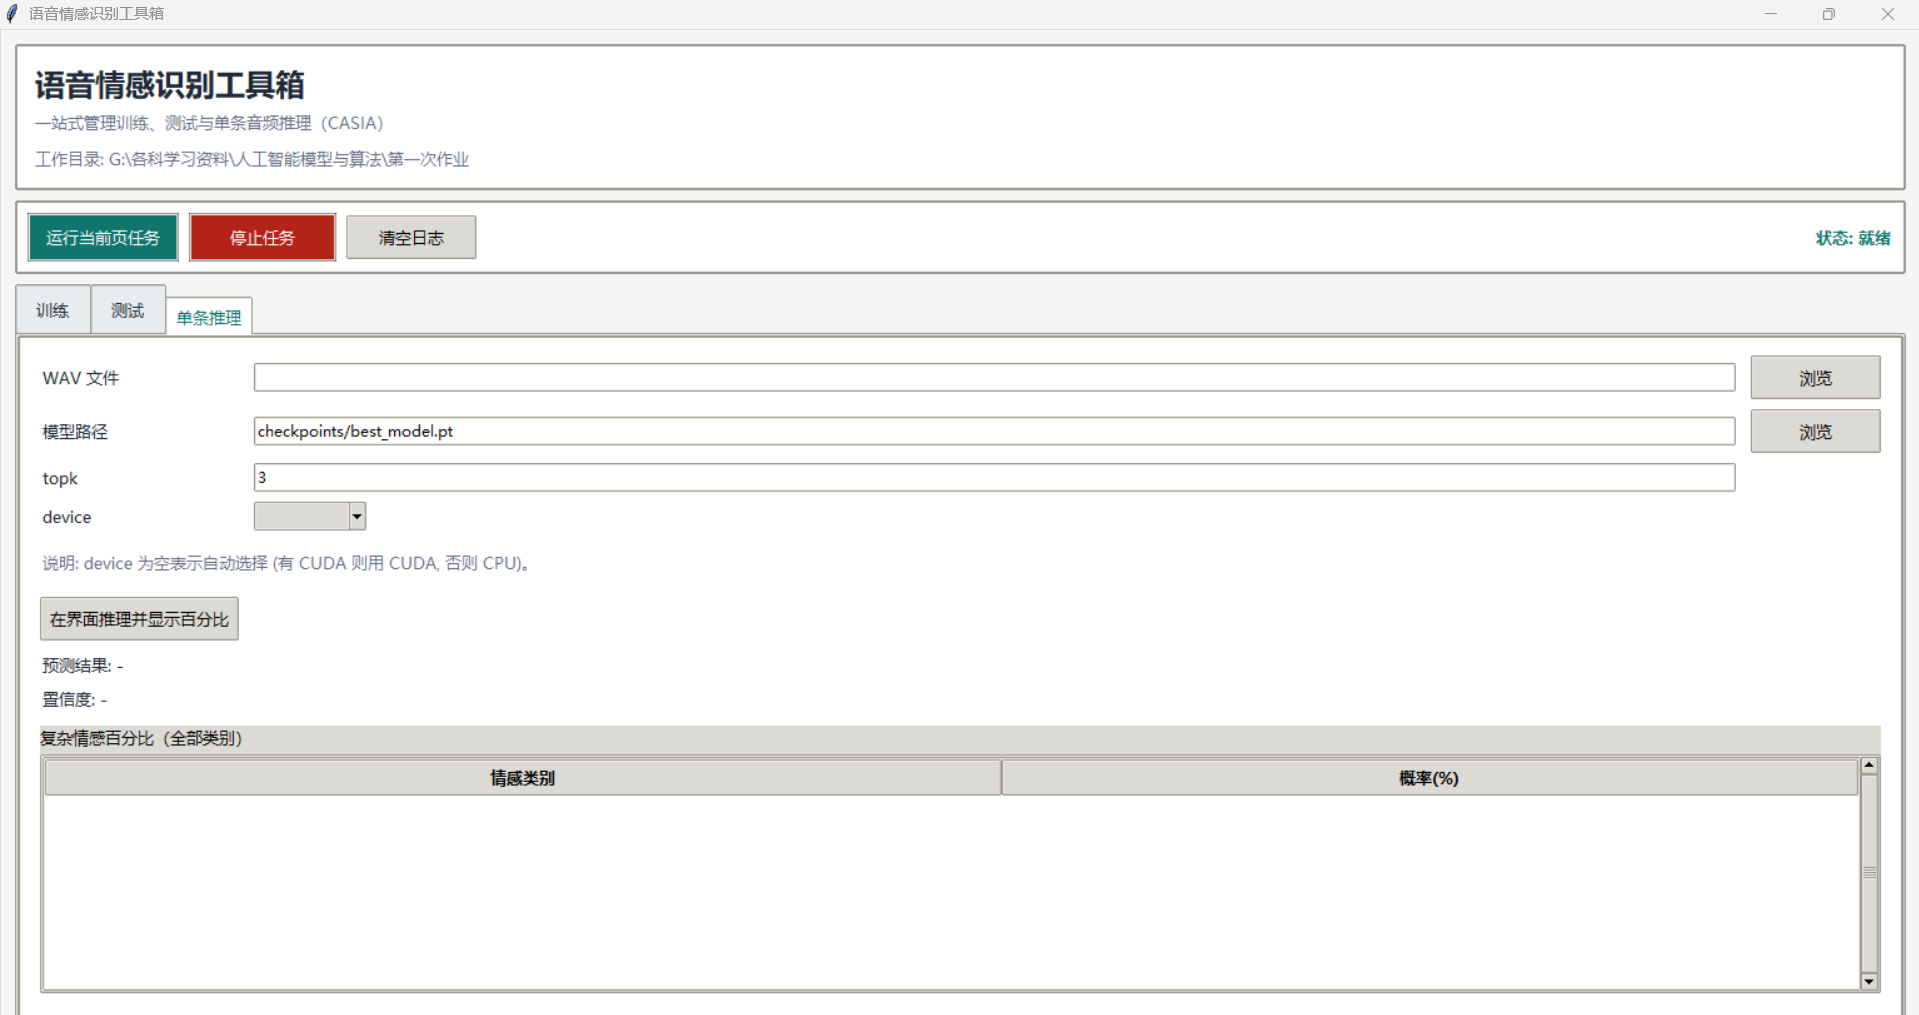
\includegraphics[width=1\linewidth]{GUI.png}
  \caption{语音情感识别系统 GUI 界面}
\end{figure}


针对上述经典语音，测试结果如下：

\begin{figure}[H]
  \centering
  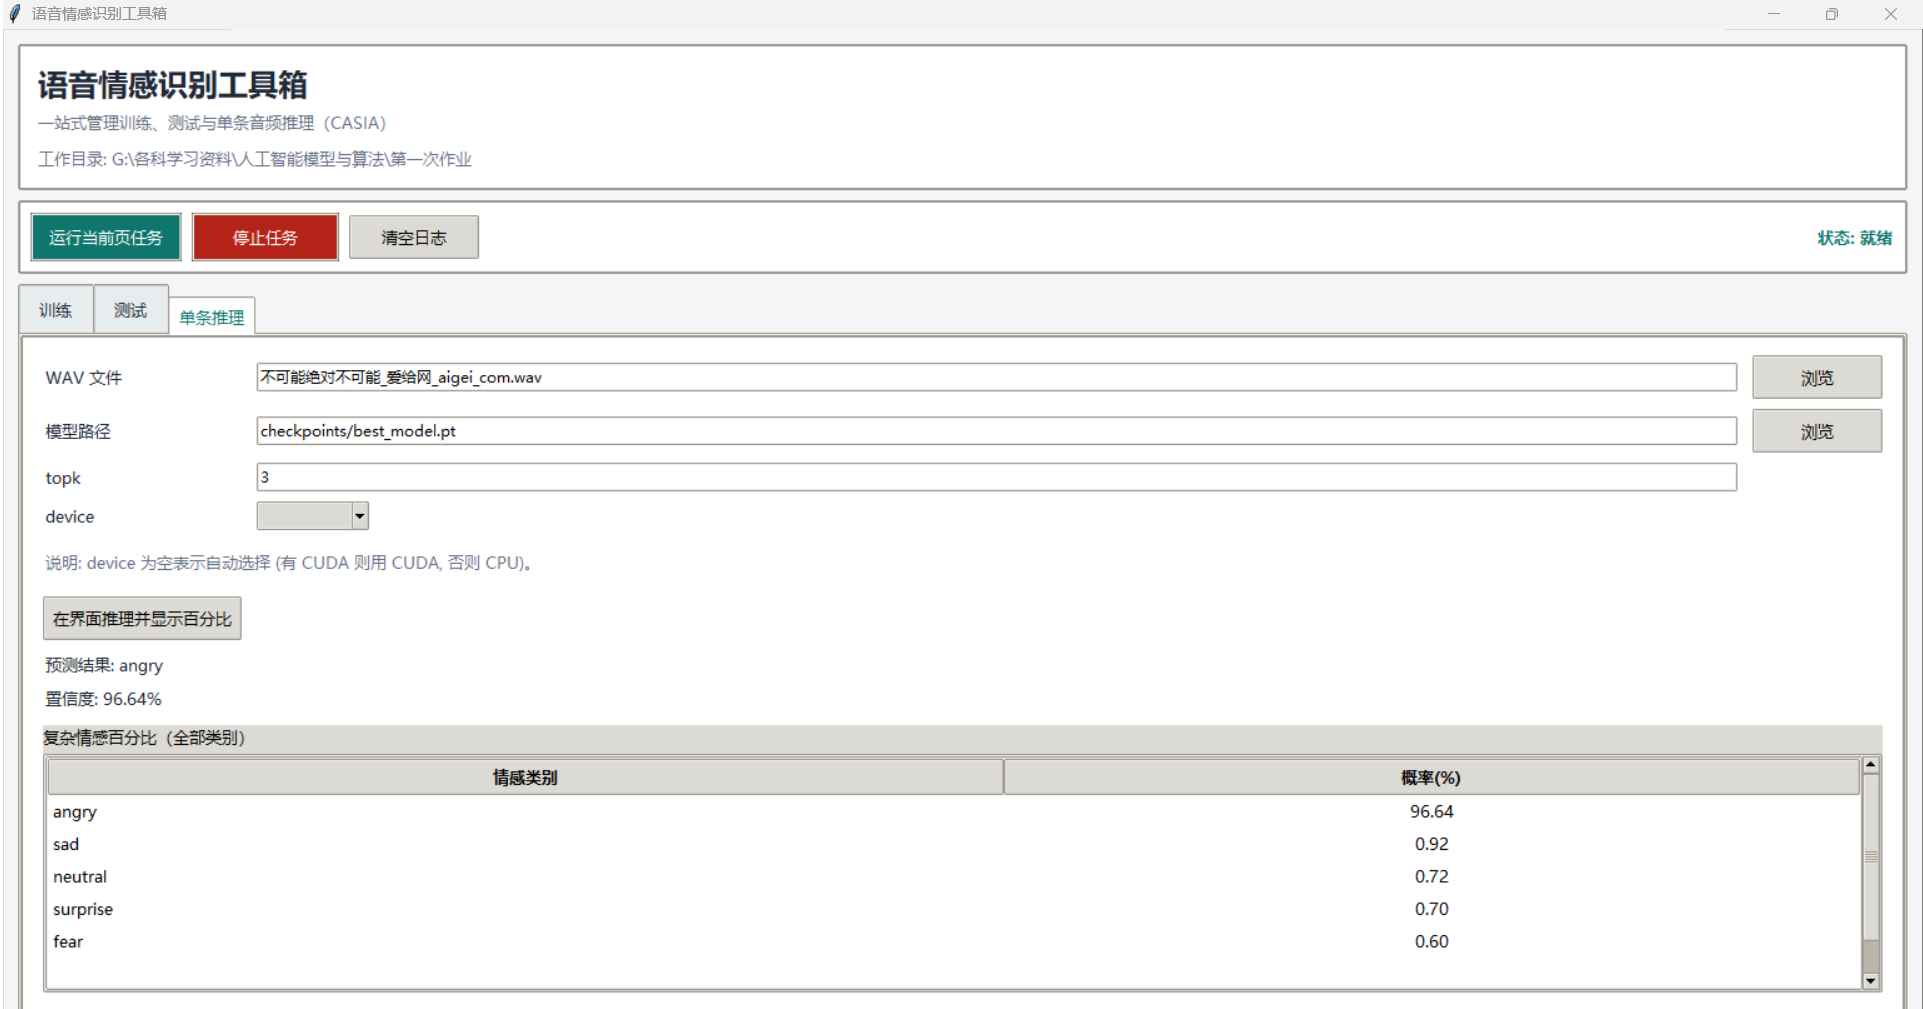
\includegraphics[width=1\linewidth]{不可能绝对不可能.png}
  \caption{“绝对不可能(曹操)”语音推理结果}
\end{figure}

\begin{figure}[H]
  \centering
  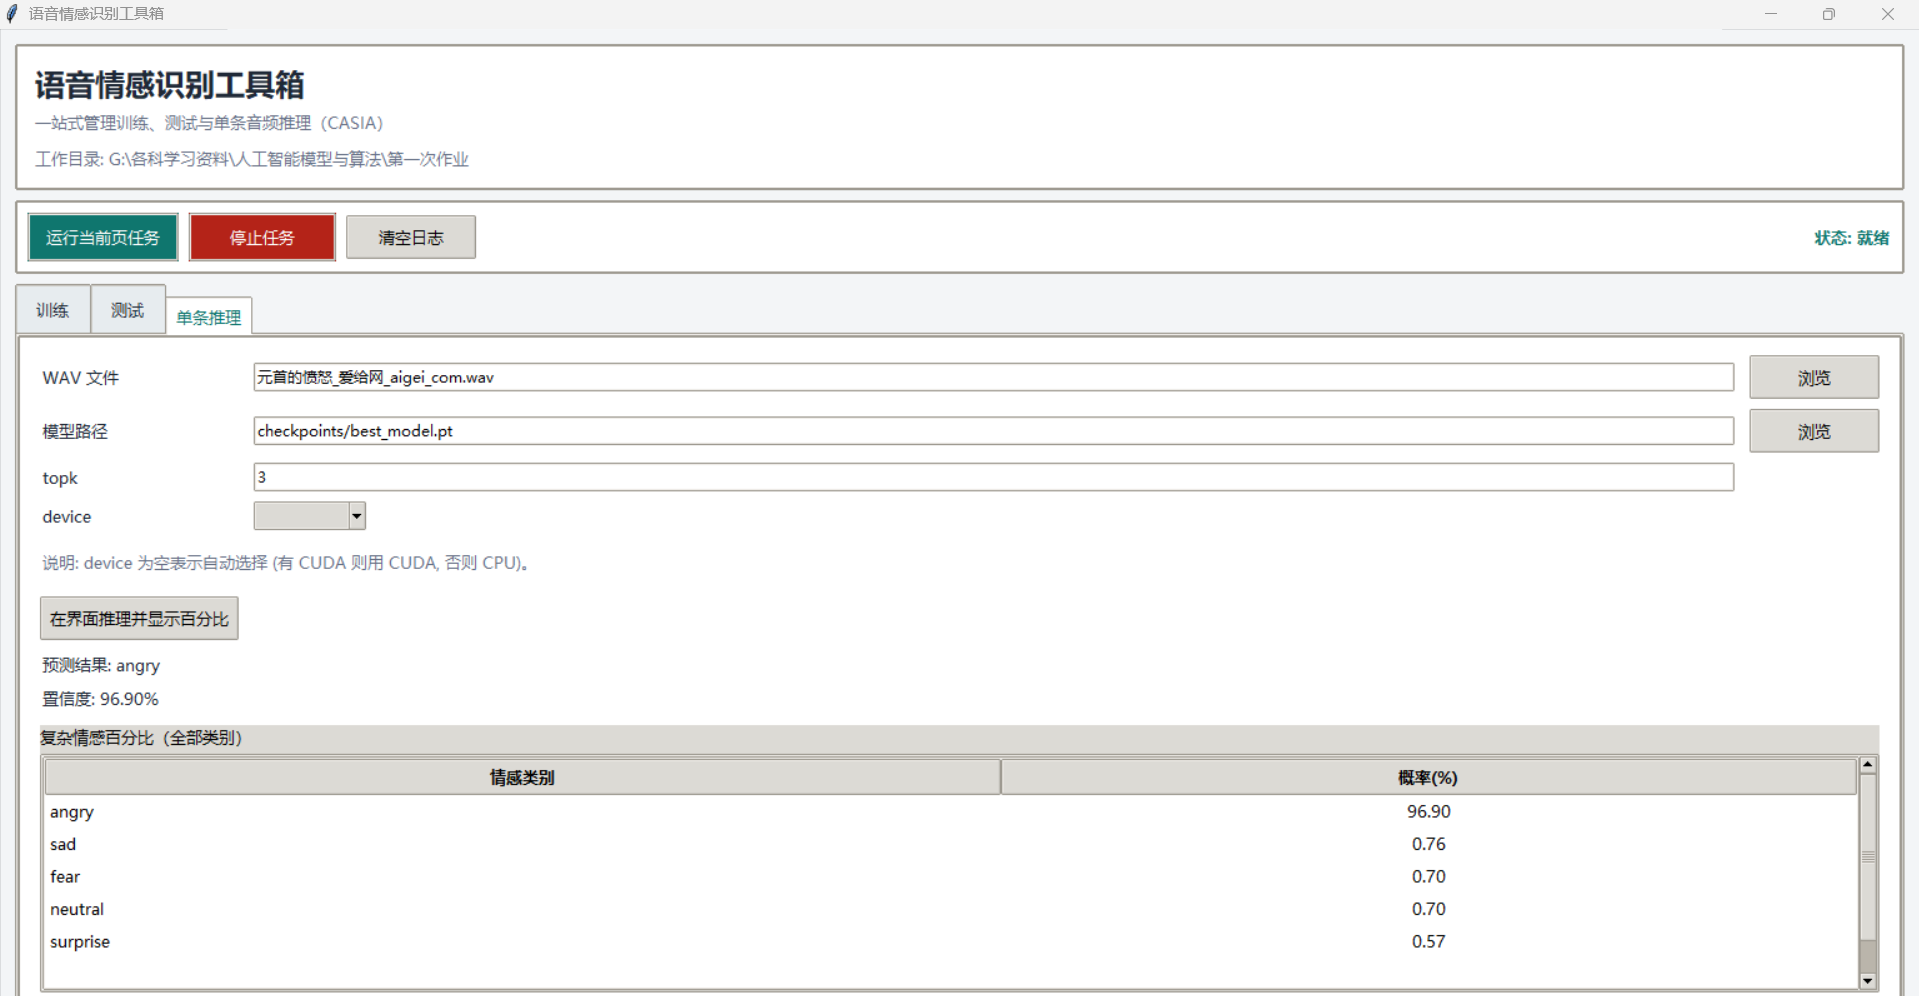
\includegraphics[width=1\linewidth]{元首的愤怒.png}
  \caption{“元首的愤怒(希特勒)”语音推理结果}
\end{figure}

\begin{figure}[H]
  \centering
  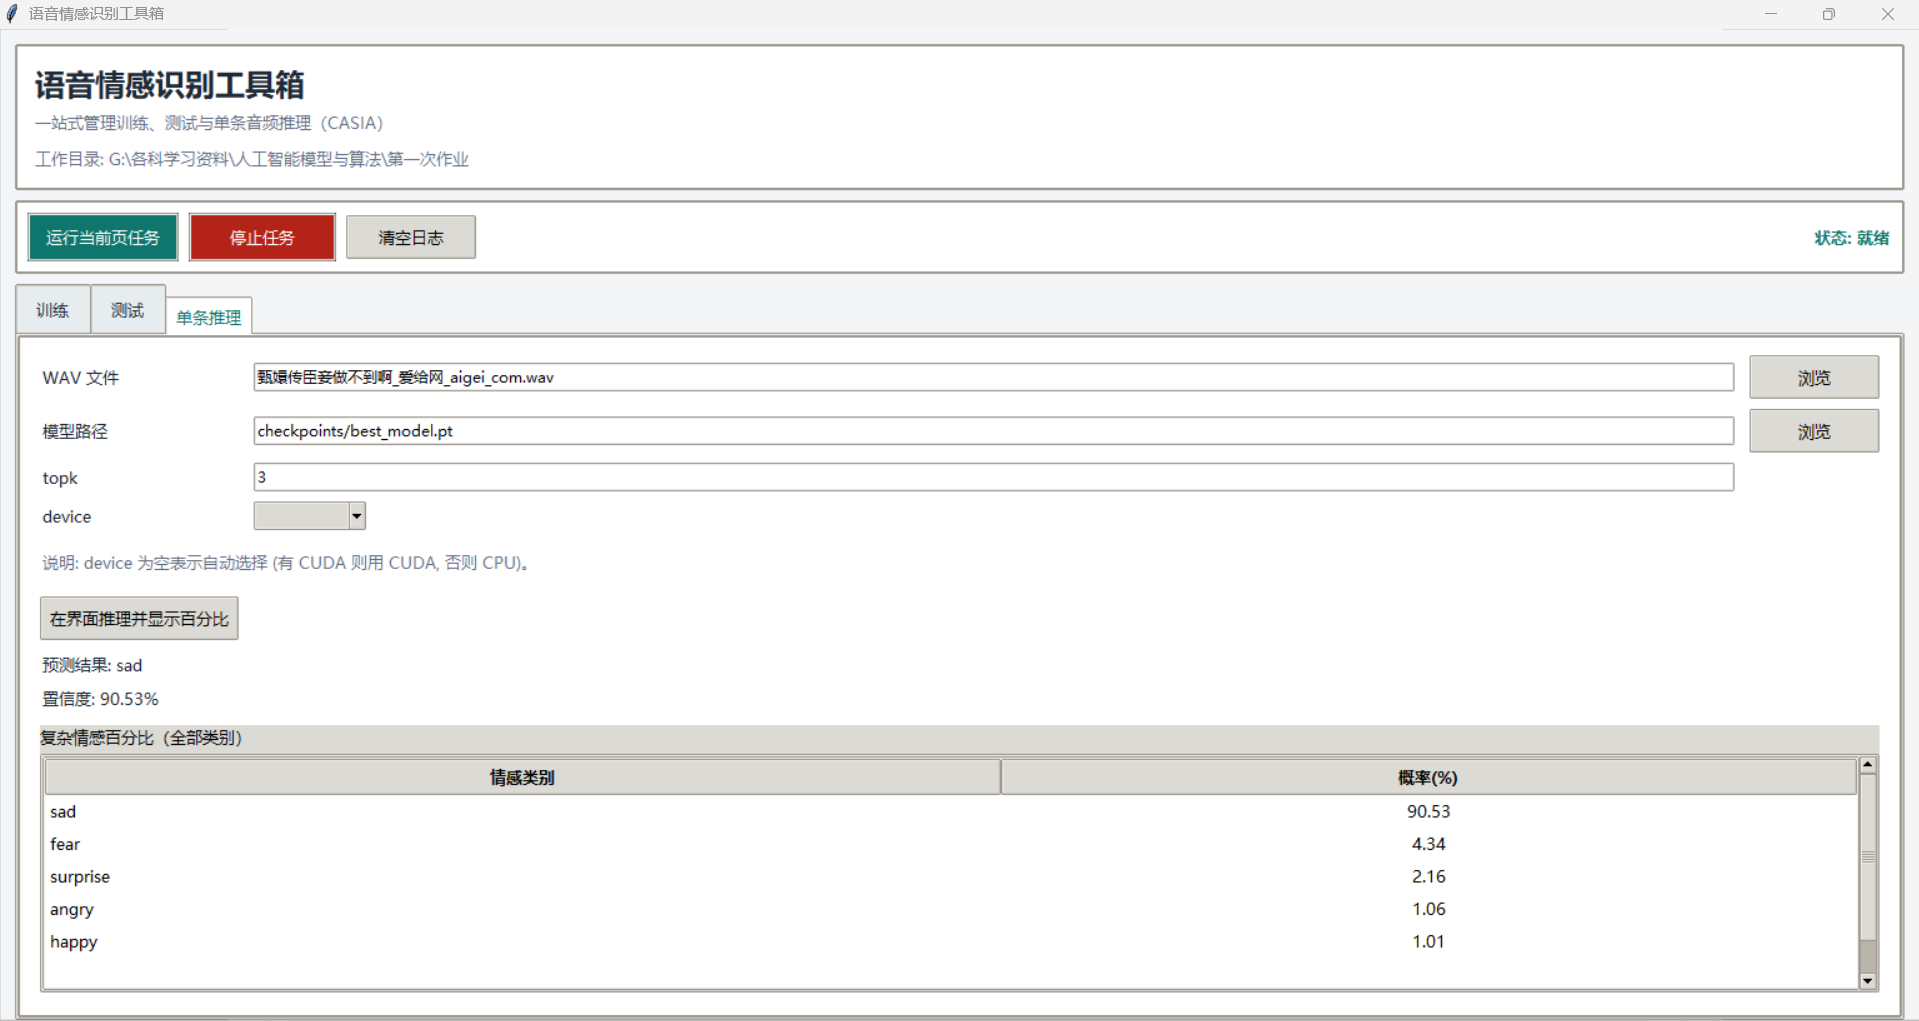
\includegraphics[width=1\linewidth]{臣妾做不到啊.png}
  \caption{“臣妾做不到啊(甄嬛传宜修)”语音推理结果}
\end{figure}

\begin{figure}[H]
  \centering
  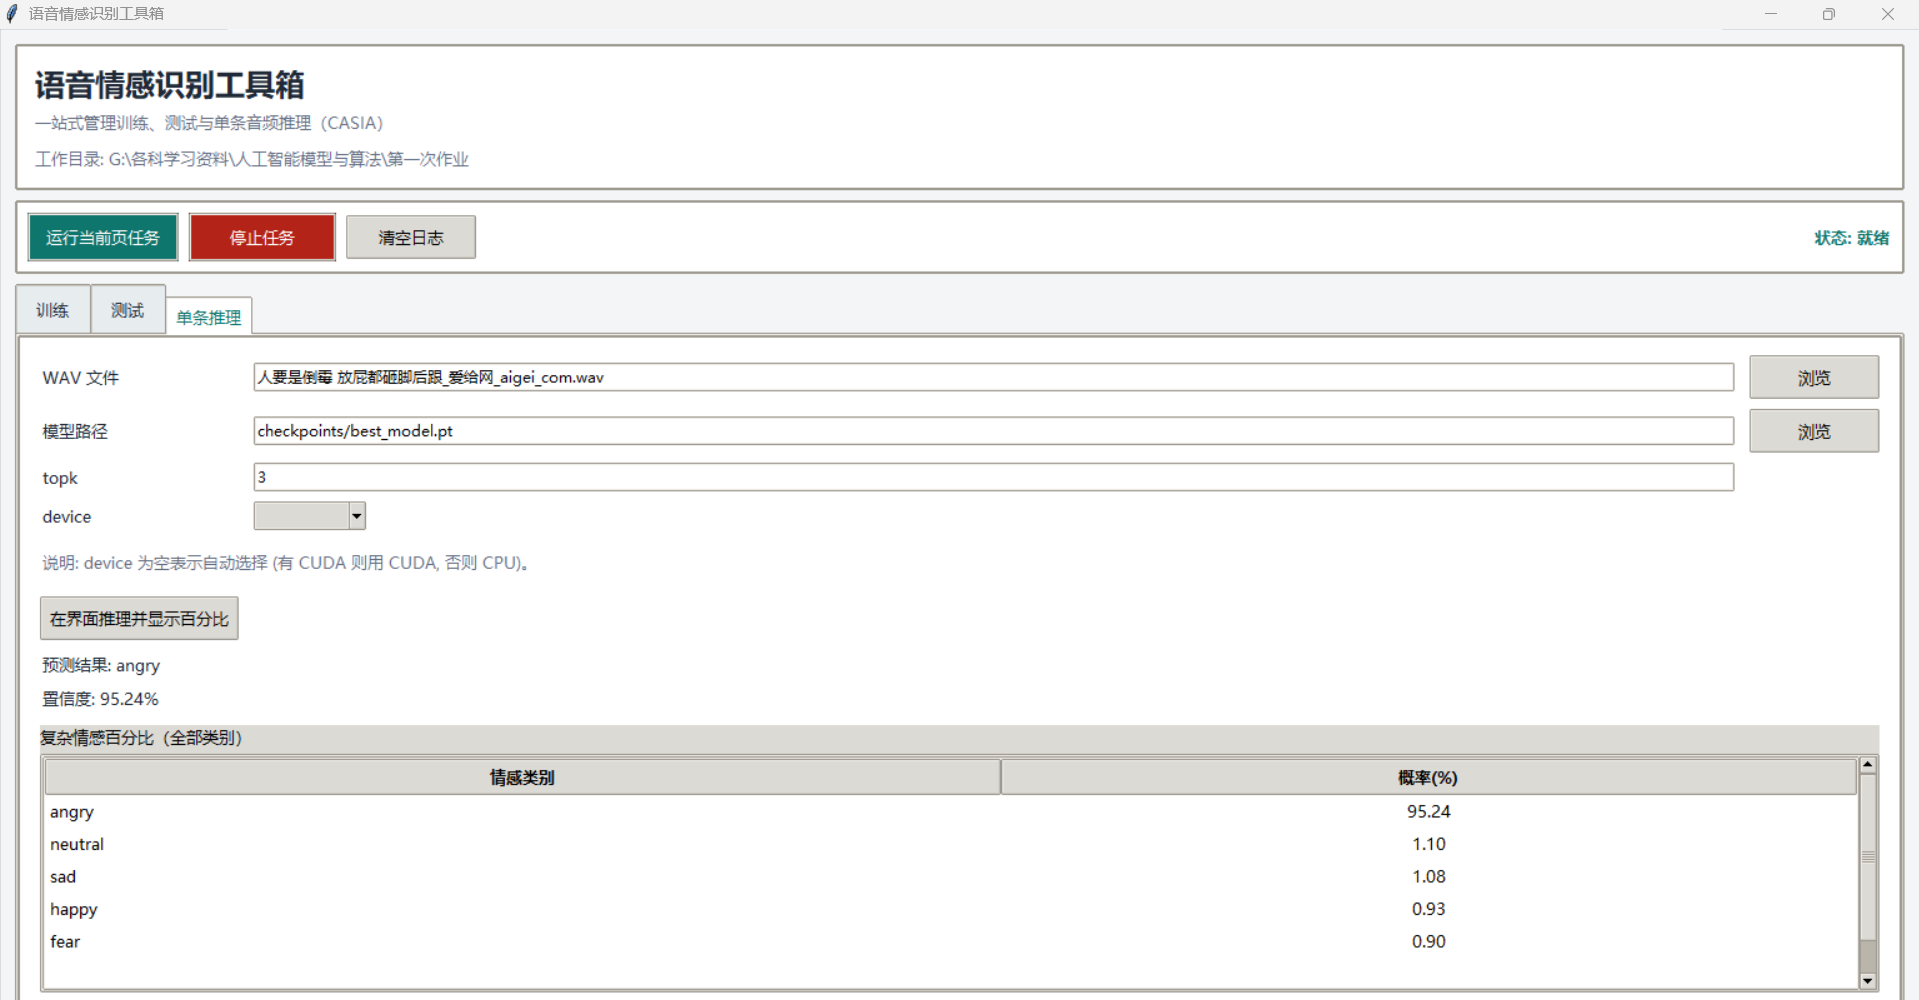
\includegraphics[width=1\linewidth]{人要是倒霉.png}
  \caption{“人要是倒霉(李云龙)”语音推理结果}
\end{figure}

\begin{figure}[H]
  \centering
  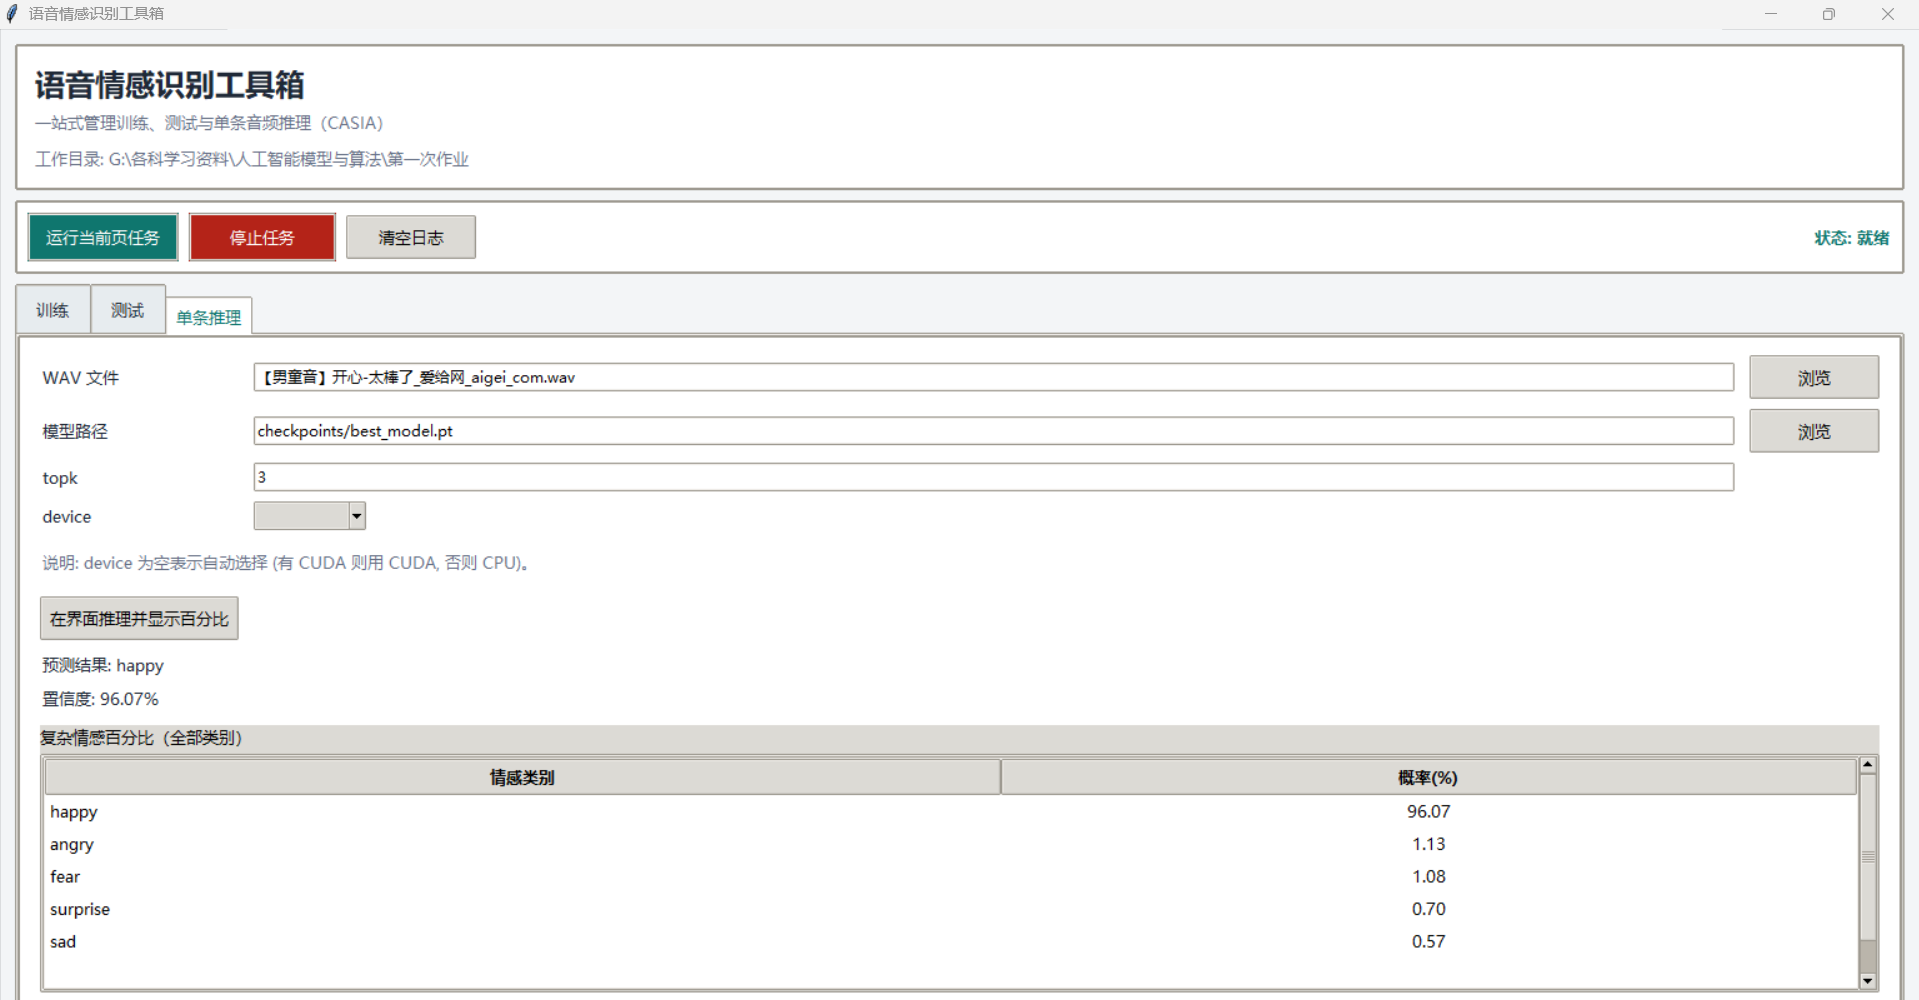
\includegraphics[width=1\linewidth]{开心太棒了.png}
  \caption{“开心太棒了(男童音)”语音推理结果}
\end{figure}

从测试截图可以看出，无论是表达愤怒、伤心还是开心等情感，模型均能给出与人类主观感受一致的分类结果，且概率分布合理，未出现明显误判。这表明本系统不仅在标准测试集上表现优异，在实际复杂语音场景下同样具备良好的实用性和鲁棒性。

\subsection{误差来源与改进分析}
误差主要来源于情感表达的模糊性与跨说话人差异。部分语音在语义上具有强烈情绪，但声学表现可能更接近中性或另一情感类别；此外，说话人音色、语速、强度与背景噪声也会影响情感特征分布。后续可通过更细粒度的情感标注、引入说话人不变特征、以及使用预训练语音表征模型进一步提升性能。



\section{局限与改进方向}
\begin{itemize}
  \item 类别不平衡：可引入更强的类别重加权或重采样。
  \item 说话人差异：对跨说话人泛化仍有提升空间。
  \item 更强的声学表征：可引入 log-Mel + delta 或预训练声学模型。
  \item 模型结构改进：尝试 Conformer、Transformer-XL 或多尺度时序建模。
\end{itemize}

\section{结论}
本项目完成了语音情感识别任务的全流程实现，从数据预处理、Transformer 模型搭建、严格划分训练评估，到 GUI 交互展示，形成了完整可复现的实验系统。在 CASIA 数据集上取得验证准确率 0.8152、测试准确率 0.7747，证明模型具备较好的情感区分能力。后续可通过更强的特征与结构设计进一步提升性能与泛化能力。


\section{主要代码与数据集说明}
\subsection{数据集：CASIA database}
CASIA 语音情感数据库采用分层文件夹结构，顶层为说话人子文件夹，次级为情感类别（angry、fear、happy、neutral、sad、surprise），底层为具体音频文件（.wav）。本项目代码可自动递归扫描该结构，兼容多说话人和多情感类别，便于扩展与复现。

\subsection{dataset.py}
\texttt{dataset.py} 负责数据集的加载、音频文件的遍历与标签推断、特征提取（Mel/MFCC）、序列长度归一化等。核心类为 \texttt{SpeechEmotionDataset}，支持灵活的数据划分与批量加载，便于与 PyTorch 训练流程集成。

\subsection{model.py}
\texttt{model.py} 实现了完整的 Transformer 编码器结构，包括输入归一化与线性映射、局部卷积前端、正弦位置编码、多层 Transformer Encoder、注意力统计池化与多层感知机分类头。代码高度模块化，便于参数调整与结构扩展。

\subsection{train.py}
\texttt{train.py} 提供训练主流程，包括数据集分层划分、模型初始化、损失函数与优化器配置、训练与验证循环、早停与模型保存、训练日志与可视化输出等。支持命令行参数灵活配置，便于实验复现。

\subsection{test.py}
\texttt{test.py} 用于模型的严格测试与单条音频推理。可加载训练好的模型权重，对指定数据划分（train/val/test）进行批量评估，输出准确率、混淆矩阵、各类别指标等，并支持单 wav 文件的情感概率推理。

\subsection{app\_gui.py}
\texttt{app\_gui.py} 基于 Tkinter 实现图形界面，集成训练、测试、推理三大功能模块。用户可通过界面选择参数、启动训练、查看日志、加载模型、选择音频文件并实时展示推理结果，极大提升了系统的易用性与演示效果。

\end{document}
